% Chapter Template

\chapter{Classic Lamination Theory and Failure Theory} % Main chapter title

\label{Chapter2} % Change X to a consecutive number; for referencing this chapter elsewhere, use \ref{ChapterX}

%----------------------------------------------------------------------------------------
%	SECTION 1
%----------------------------------------------------------------------------------------

\section{Classic Lamination Theory}
A laminate is consist of multiple laminas bonded together through thickness. In
this chapter, first the stress-strain relationship is developed based on Hook's
law for a single lamina; second, develop relationship of mechanical loads
applied to a laminate to strains and stresses in each lamina, calculate the
elastic moduli of laminate based on the elastic moduli of single laminate and
the lay-up..


\subsection{Analysis of stress and strain for composite material}

\begin{figure*}[!htb]
	\centering
	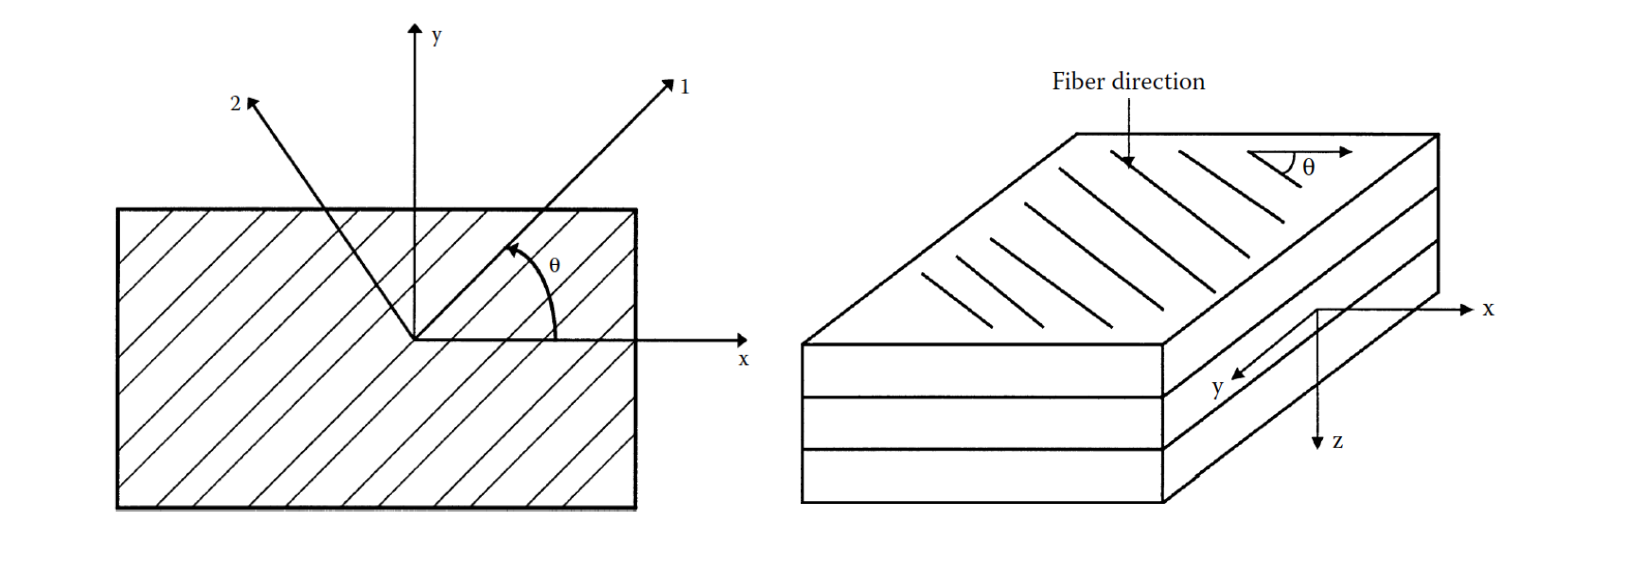
\includegraphics[width=\linewidth]{../../image/laminate_design/lamina_local_global_axes.png}
\caption{Lamina}
  	\label{fig:lamina}
\end{figure*}

\subsection{Stress and Strain in a Lamina}
For a single lamina has a small thickness under plane stress, and it's upper and lower surfaces of the lamina are
free from external loads. According to the Hooke's Law, the three-dimensional stress-strain equations can be reduced to
two-dimensional stress-strain equations. The stress-strain relation in local axis 1-2 is
\begin{equation}
    \begin{bmatrix}
        \sigma _1\\
        \sigma _2\\
        \tau_{12}
    \end{bmatrix}
    =
    \begin{bmatrix}
        Q_{11} & Q_{12} & 0\\
        Q_{12} & Q_{22} & 0\\
        0      &  0     & Q_{66}
    \end{bmatrix}
    \begin{bmatrix}
        \varepsilon_1\\
        \varepsilon_2\\\gamma_{12}
	\end{bmatrix}_{\textstyle .} 
\end{equation}
where $Q_{ij} $are the stiffnesses of the lamina that are related

to engineering elastic constants given by
\begin{equation}
    \begin{split}
	&Q_{11}=\frac{E_1}{1-v_{12}v_{21}},\\
	&Q_{22}=\frac{E_2}{1-v_{12}v_{21}},\\
	&Q_{66}=G_{12},\\
	&Q_{12}=\frac{v_{21}E_2}{1-v_{12}v_{21}},\\
    \end{split}
\end{equation}

where $E_1, E_2, v_{12}, G_{12} $ are four independent engineering elastic constants, which are defined as follows: $E_1 $ is the longitudinal Young's modulus, $E_2 $ is the transverse Young's modulus, $v_{12} $ is the major Poisson's ratio, and $G_{12} $ is the in-plane shear modulus.

Stress strain relation in the global x-y axis is
\begin{equation}\left[\begin{array}{l}\sigma _{x} \\ \sigma _{y} \\
	\tau_{xy}\end{array}\right]=\left[\begin{array}{lll}\bar{Q}_{11} &
\bar{Q}_{12} & \bar{Q}_{16}\\ \bar{Q}_{12} & \bar{Q}_{22} & \bar{Q}_{26} \\
\bar{Q}_{16} & \bar{Q}_{26}
			 &\bar{Q}_{66}\end{array}\right]\left[\begin{array}{l}\varepsilon_{x}
	 \\ \varepsilon_{y}\\ \gamma_{x y}\end{array}\right]_{\textstyle ,}
\end{equation}
where

\begin{equation}
	\begin{array}{l}
		\resizebox{.55\textwidth}{!}{$\bar{Q}_{11}=Q_{11} cos^{4}\theta+Q_{22} sin^{4}\theta+2\left(Q_{12}+2
		Q_{66}\right) sin^{2}\theta cos^{2}\theta$}, \\

		\resizebox{.55\textwidth}{!}{$\bar{Q}_{12}=\left(Q_{11}+Q_{22}-4 Q_{66}\right) sin^{2}\theta
		cos^{2}\theta+Q_{12}\left(cos^{4}\theta+sin^{2}\theta \right)$}, \\

		\resizebox{.55\textwidth}{!}{$\bar{Q}_{22}=Q_{11} sin^{4}\theta+Q_{22} cos^{4}\theta+2\left(Q_{12}+2
		Q_{66}\right) sin^{2}\theta cos^{2}\theta$}, \\

		\resizebox{.6\textwidth}{!}{$\bar{Q}_{16}=\left(Q_{11}-Q_{12}-2
		Q_{66}\right) cos^{3}\theta sin\theta-\left(Q_{22}-Q_{12}-2Q_{66}\right)
	sin^{3}\theta cos\theta$}, \\ 
		\resizebox{.6\textwidth}{!}{$\bar{Q}_{26}=\left(Q_{11}-Q_{12}-2
		Q_{66}\right) cos\theta sin^{3}\theta-\left(Q_{22}-Q_{12}-2
Q_{66}\right)cos^{3}\theta sin\theta$},
		 \\ 
	\resizebox{.6\textwidth}{!}	{$\bar{Q}_{66}=\left(Q_{11}+Q_{22}-2 Q_{12}-2 Q_{66}\right)
	sin\theta^{2}cos\theta^{2}+Q_{66}\left(sin\theta^{4}+cos\theta^{4}\right)$}.\\
	\end{array}
\end{equation}


The local and global stresses in an angle lamina are related

to each other through the angle of the lamina $\theta $, it can be written as 
\begin{equation}
	\left[\begin{array}{l}\sigma _{1} \\ \sigma _{2} \\
	\tau_{12}\end{array}\right]=[T]\left[\begin{array}{l}\sigma _{x} \\ 
	\sigma _{y} \\\tau_{xy}\end{array}\right]_{\textstyle ,}
\end{equation}

where
\begin{equation}
	[T]=\left[\begin{array}{ccc}cos^{2}\theta & sin^{2}\theta & 2
		sin\theta cos\theta \\ 
sin^{2}\theta & cos^{2}\theta & -2 sin\theta cos\theta \\
-sin\theta cos\theta
			  & sin\theta cos\theta  &cos^{2}\theta -sin^{2}\theta
\end{array}\right]_{\textstyle .} 
\end{equation}



\subsection{Stress and Strain in a Laminate}
For forces and moment resultants acting on laminates, such as in plate and shell
structures, the relationship between applied forces and moment and displacement
can be given by

\begin{equation} \label{eq:force_and_moments}
	\begin{array}{l}
		\begin{aligned}
	\begin{bmatrix}
		N_x \\
		N_y \\
		N_{xy}
	\end{bmatrix}
	&=
	\begin{bmatrix}
		A_{11} & A_{12} & A_{16} \\
		A_{12} & A_{22} & A_{26} \\
		A_{16} & A_{26} & A_{66} 
	\end{bmatrix}
    \begin{bmatrix}
		\varepsilon_x^0 \\
        \varepsilon_y^0 \\
		\gamma_{xy}^0
    \end{bmatrix}   \\
	&+               
	\begin{bmatrix}
		B_{11} & B_{12} & B_{16} \\
		B_{11} & B_{12} & B_{16} \\
		B_{16} & B_{26} & B_{66} 
	\end{bmatrix}
	\begin{bmatrix}
		k_x \\
		k_y \\
		k_{xy} 
	\end{bmatrix}_{\textstyle ,}  \\
\end{aligned} \\ \\
\begin{aligned}
	\begin{bmatrix}
		M_x \\
		M_y \\
		M_{xy}
	\end{bmatrix}
	&=
	\begin{bmatrix}
		B_{11} & B_{12} & B_{16} \\
		B_{12} & B_{22} & B_{26} \\
		B_{16} & B_{26} & B_{66} 
	\end{bmatrix}
    \begin{bmatrix}
		\varepsilon_x^0 \\
        \varepsilon_y^0 \\
		\gamma_{xy}^0
    \end{bmatrix} \\ 
	&+  
	\begin{bmatrix}
		D_{11} & D_{12} & D_{16} \\
		D_{11} & D_{12} & D_{16} \\
		D_{16} & D_{26} & D_{66} 
	\end{bmatrix}
	\begin{bmatrix}
		k_x \\
		k_y \\
		k_{xy} 
	\end{bmatrix}_{\textstyle,}
\end{aligned}
	\end{array}
\end{equation}

where

$N_x,N_y $  - normal force per unit length;

$N_{xy} $  - shear force per unit length;

$M_x, M_y $ - bending moment per unit length;

$M_{xy} $  - twisting moments per unit length;

$\varepsilon^{0}, k $- mid plane strains and curvature of a laminate in x-y
coordinates.

The mid plane strain and curvature is given by
\begin{equation}
    \begin{split}
    &A_{ij}=\sum_{k=1}^{n}(\overline{Q_{ij}})_k(h_k-h_{k-1})  i=1,2,6, j=1,2,6,\\
    &B_{ij}=\frac{1}{2}\sum_{k=1}^{n}(\overline{Q_{ij}})_k(h_k^2 - h_{k-1}^2)
	i=1,2,6, j=1,2,6,\\
    &D_{ij}=\frac{1}{3}\sum_{k=1}^{n}(\overline{Q_{ij}})_k(h_k^3 - h_{k-1}^3)
	i=1,2,6, j=1,2,6.\\
    \end{split}
\end{equation}

The [A], [B], and [D] matrices are called the extensional, coupling, and bending stiffness matrices,
respectively. The extensional stiffness matrix $[A]$ relates the resultant in-plane forces to the
in-plain strains, and the bending stiffness matrix $[D]$ couples the resultant bending moments to
the plane curvatures.  The coupling stiffness matrix $[B]$ relates the force and moment terms to the
midplain strains and midplane curvatures.

\section{Failure Theory}

Failure criteria for composite materials are more difficult to predict due to
structural and material complexity in comparison to isotropic materials. The
failure process of a composite materials can be regarded from microscopic and
macroscopic points of view. Most popular criteria about the failure of an angle
lamina are in terms of macroscopic failure criteria, which are based on the
tensile, compressive and shear strengths. According to the failure surfaces,
these criteria can be classified into two classes: one is called independent
failure mode criteria which includes the maximum stress failure theory, maximum
strain failure theory because their failure envelop are rectangle; another is
called quadratic polynomial which includes Tsai-Wu, Chamis, Hoffman and Hill
criteria because their failure surfaces are of ellipsoidal shape. In the present
study, two most reliable failure criteria is taken, Maximum stress and Tsai-wu.
Both of these two failure criteria are based on the stresses in the local axes
instead of principal normal stresses and maximum shear stresses, and four normal
strength parameters and one shear stress for a unidirectional lamina are
involved. The five strength parameters are

$(\sigma _1^{T})_{ult}= $ ultimate longitudinal tensile strength(in direction 1),

$(\sigma _1^{C})_{ult}= $ ultimate longitudinal compressive strength,

$(\sigma _2^{T})_{ult}= $ ultimate transverse tensile strength,

$(\sigma _2^{C})_{ult}= $ ultimate transverse compressive strength, and

$(\tau_{12})_{ult}= $ and ultimate in-plane shear strength.

\begin{figure}
\centering
\begin{tikzpicture}
	\begin{scope}
		%\draw[style=help lines] (-3,-3) grid (3,3);
		\draw (0,0) rectangle (2,3);
		\draw[->] (1.3,1.2) -- (2.6,1.2);
		\draw[->] (1.3,1.2) -- (1.3,3.4);
		\node at (2.2,1) {$X_T$};
		\node at (1.5, 3.2) {$Y_T$};
		\node at (-0.2, 0.9) {$X_C$};
		\node at (1.8, -0.2) {$Y_C$};
	\end{scope}
	\begin{scope}[xshift=6cm,yshift=1.15cm]
		%\draw[style=help lines] (-3,-3) grid (3,3);
		\draw[rotate=30] (0,0) ellipse (2cm and 1cm);
		\draw[->] (0.2,0) -- (0.2,2.2);
		\draw[->] (0.2,0) -- (1.9,0);
		\node at (1.6,-0.2) {$X_T$};
		\node at (0.3, 1.3) {$Y_T$};
		\node at (-1.6, 0) {$X_C$};
		\node at (-0.5, -1.5) {$Y_C$};
	\end{scope}
\end{tikzpicture}
\caption{Schematic failure surfaces for maximum stress and quadratic failure
criteria}
\end{figure}


\subsection{Tsai-wu failure criterion}
The TW criterion is one of the most reliable static failure criteria which is derived from the von
Mises yield criterion.  
A lamina is considered to fail
if \begin{equation} \label{eq:tsai_wu}
\begin{split}
	H_1 \sigma_1  & + H_2 \sigma_2 + H_6 \tau_{12} + H_{11}\sigma_1^2 + H_{22} \sigma_2^2 \\
				  & + H_{66}  \tau_{12}^2 + 2H_{12}\sigma_1\sigma_2 < 1
\end{split}
\end{equation}

is violated, where

\begin{equation}
	\begin{split}
		H_{1}&=\frac{1}{\left(\sigma_{1}^{T}\right)_{u l
		t}}-\frac{1}{\left(\sigma_{1}^{C}\right)_{u l t}} \textstyle{,} \\
		H_{11}&=\frac{1}{\left(\sigma_{1}^{T}\right)_{u l t}\left(\sigma_{1}^{C}\right)_{u l t}} \textstyle{,}\\
		H_{2}&=\frac{1}{\left(\sigma_{2}^{T}\right)_{u l t}}-\frac{1}{\left(\sigma_{2}^{C}\right)_{u l t}} \textstyle{,}\\
		H_{22}&=\frac{1}{\left(\sigma_{2}^{T}\right)_{u l t}\left(\sigma_{2}^{C}\right)_{u l t}} \textstyle{,}\\
		H_{66}&=\frac{1}{\left(\tau_{12}\right)_{u l t}^{2}} \textstyle{,}\\
		H_{12}&=-\frac{1}{2} \sqrt{\frac{1}{\left(\sigma_{1}^{T}\right)_{u l
		t}\left(\sigma_{1}^{C}\right)_{u l t}\left(\sigma_{2}^{T}\right)_{u l
		t}\left(\sigma_{2}^{C}\right)_{u l t}}}\textstyle{.}
	\end{split}
\end{equation}

$H_i$ is the strength tensors of the second order; $H_{ij}$ is the strength
tensors of the fourth order. $\sigma_1$ is the applied normal stress in 
direction 1; $\sigma_2$ is the applied normal stress in the direction 2; and
$\tau_{12}$ is the applied in-plane shear stress.




\subsection{Maximum Stress Failure Theory}

Maximum stress(MS) failure theory consists of maximum normal stress theory
proposed by Rankine and maximum shearing stress theory by Tresca. The stresses
applied on a lamina can be resolved into the normal and shear stresses in the
local axes. If any of the normal or shear stresses in the local axes of a lamina
is equal or exceeds the corresponding ultimate strengths of the unidirectional
lamina, the lamina is considered to be failed. That is

$\sigma_1 \geq (\sigma _1^{T})_{ult} $ or $\sigma_1 \leq -(\sigma _1^{C})_{ult}
$,

$\sigma_2 \geq (\sigma _2^{T})_{ult} $ or $\sigma_2 \leq -(\sigma _2^{C})_{ult}
$,

$\tau_{12} \geq (\tau_{12})_{ult} $  or $\tau_{12} \leq -(\tau_{12})_{ult} $.

where $\sigma_1$ and $\sigma_2$ are the normal stresses in the local axes 1 and 2, respectively;
$\tau_{12}$ is the shear stress in the symmetry plane 1-2.
The safety factor, or yield stress, is how much extra load beyond is intended a
composite laminate will actually take, which is an indication of the material's
load carrying capacity. If the value is less then 1.0, it means failure. The safey factor is defined as 

\begin{equation} \label{eq:sr}SF=\frac{\text {Maximum Load Which Can Be
	Applied}}{\text {Load Applied}} {\textstyle .}
\end{equation}

The safety factor based on maximum stress theory is calculated by the following
method: first, the principal stresses($\sigma_1^k$,$\sigma_2^k$, and
$\tau_{12}^k$) are obtained by experiment; evaluate the safety factor along each
direction according to equation \ref{eq:sr}; The minimum value among these
safety factors are denoted as the safety factor of the lamina, $SF_{MS}^k$, it
can be written as 

\begin{align}
	SF_{MS}^k = \text{min of}
	\begin{cases}
		SF_X^k = 
		\begin{cases}
			\frac{X_t}{\sigma_{11}}, \text{ if } \sigma_{11}>0 \\
			\frac{X_c}{\sigma_{11}}, \text{ if } \sigma_{11}<0 \\
		\end{cases} \\
		SF_Y^k = 
		\begin{cases}
			\frac{Y_t}{\sigma_{22}}, \text{ if } \sigma_{22}>0 \\
			\frac{Y_c}{\sigma_{22}}, \text{ if } \sigma_{22}<0 \\
		\end{cases} \\
		SF_S^k =
		\begin{cases}
			\frac{S}{|\tau_{12}|} \\
		\end{cases} \\
	\end{cases} \textstyle{.}
\end{align}


Assuming the composite laminate under a in-plane loading f, the corresponding
stress on local stress in direction 1, local stress in direction 2, and shear
stress for the kth lamina are $\sigma_1 SF_{TW}^k$, $\sigma_2SF_{TW}^k$, and $\tau_{12}SF_{TW}^k$,
respectively. Substitute them into the equation \ref{eq:tsai_wu}, the expression
are given by

$a(SF_{TW}^k)^2 + b(SF_{TW}^k) - 1 = 0 \textstyle{,}$

where 


$a = H_{11}(\sigma_1)^2 + H_{22}(\sigma_2)^2 +H_{66}(\tau_{12})^2 +
2H_{12}\sigma_1 \sigma_2 \textstyle{,} $


$b = H_1\sigma_1 + H_2 \sigma_2 + H_6 \tau_{12} \textstyle{.}$ 


Solve the above equation, the safety factor for the kth lamina is 

$SF_{TW}^k = |\frac{-b+ \sqrt{b^2 + 4a}}{2a}|$.

Then, the minimum of $SF_{TW}^k$ is taken as the safety factor of the
laminate which is written as

$SF_{TW}= \text{ min of } SF_{TW}^k \text{ for } k=1,2,\cdots, m-1,m$ .



\section{Summary}
In this chapter, we review the CLT for composite material's analysis, then
related failure theories are introduced to check whether a composite material
would fail or not. In the following chapters, the CLT would be used to
calculate the stress and strain under in-plane loading, it would also be used
to generate the training data for stress and strain approximation based on
neural network; in order to design a proper composite material, the failure theory 
are used to decide the feasibility of composite design.
